\documentclass[tikz, border=2pt]{standalone}

\usepackage{helvet}
\renewcommand{\familydefault}{\sfdefault}

\usepackage[EULERGREEK]{sansmath}
\sansmath
\usetikzlibrary{arrows.meta}

\begin{document}%

\begin{tikzpicture}[line width=2pt]
\tikzset{>={Latex[width=3mm,length=4mm]}}

% grid
\draw[help lines] (-2, -5) grid (10, 5);


\node[inner sep=0pt] (figa) at (0.5,0)
{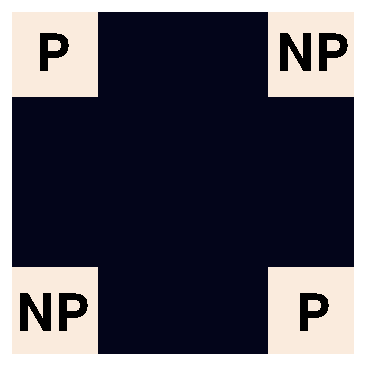
\includegraphics[width=0.2\textwidth]{./pop_icon_2.pdf}};

\draw [-, line width=1.5pt, black] (2,0) -- (3.99,0);

\draw [dotted, line width=1.5pt, black] (4,0) -- (5,0);

\draw [->, line width=1.5pt, black] (5,0) -- (7.,0);

\draw [-, line width=1.5pt, black] (2,-0.025) -- (2,0.5);

\draw [-, line width=1.5pt, black] (3,-0.025) -- (3,0.5);

\draw [-, line width=1.5pt, black] (4,-0.025) -- (4,0.5);

\draw [-, line width=1.5pt, black] (5,-0.025) -- (5,0.5);

\draw [-, line width=1.5pt, black] (6,-0.025) -- (6,0.5);

% \draw (-2.2, 2.2) node{{\Huge\sf\textbf{P}}};
% \draw (2.2, 2.2) node{{\Huge\sf\textbf{NP}}};
% \draw (2.2, -2.2) node{{\Huge\sf\textbf{P}}};
% \draw (-2.2, -2.2) node{{\Huge\sf\textbf{NP}}};

% \draw [-, line width=1.5pt, black] (-3, 2.9) -- (-3.5, 2.9) -- (-3.5, -2.9) -- (-3, -2.9); 

% \draw [-, line width=1.5pt, black] (-2.9, -3.) -- (-2.9, -3.5) -- (2.9, -3.5) -- (2.9, -3.); 

\node at (2.5,0.3) [draw=none, rectangle, rotate=0] (g1) {\sf \small Env I};

\node at (3.5,0.3) [draw=none, rectangle, rotate=0] (g1) {\sf \small Env II};

\node at (5.5,0.3) [draw=none, rectangle, rotate=0] (g1) {\sf \small Env I};

% \node at (0,-3.5) [draw=none, rectangle, rotate=0, fill=white] (g1) {\sf \huge $m=10$};
% %labels


\end{tikzpicture}


\end{document}